%%
%% Generated by gpt_translate from demo/theorie.tex, on 2024-07-09 16:48:40 using model gpt-3.5-turbo-16k
%%

% GPT CHUNK%
\documentclass{ximera}
%\documentclass[handout]{ximera}
\input{../preamble.tex}
\addPrintStyle{..}

\begin{document}
    \author{Wim Obbels}
    \xmtitle{Example Theory Module}{A simple Ximera module}
    \label{xim:ximeraDemo}

This is an example of a theory module in Ximera, 
with some useful \texttt{environment}s and \texttt{command}s.


% Demo about not completely equalizing PDF and HTML ... !
\pdfOnly{
    \begin{remark}\nl 
        It is advisable to also view the Online version. 
        For example, it will become clear that this remark has been replaced by the suggestion to also consult the PDF.

    \ifhandout
       By the way, you are using the \textit{handout} PDF, which does not contain answers.

       There is also a so-called \textit{standard} PDF \textit{which does contain answers and hints}.
    \else
      You are, by the way, using the so-called \textit{standard} PDF, which contains the answers to the exercises.

      There is also a \textit{handout} PDF \textit{without the answers}.
    \fi

\end{remark}
    }

\begin{onlineOnly}
 \begin{remark}
    It is advisable to also view the PDF version. 
    For example, it will become clear that this suggestion has been replaced by the suggestion to consult the Online version.
 \end{remark}
\end{onlineOnly}



You can experiment with an interactive graph of the cosine function (via Desmos):
\[  
\graph[xmin=-5,xmax=20,ymin=-1,ymax=1]{y=cos(x)}  
\] 
\pdfOnly{
but because you are using the PDF version, that of course does not work, 
and we only show a rather \textit{boring} graph with tikz here:

\begin{image}[0.7\textwidth]
    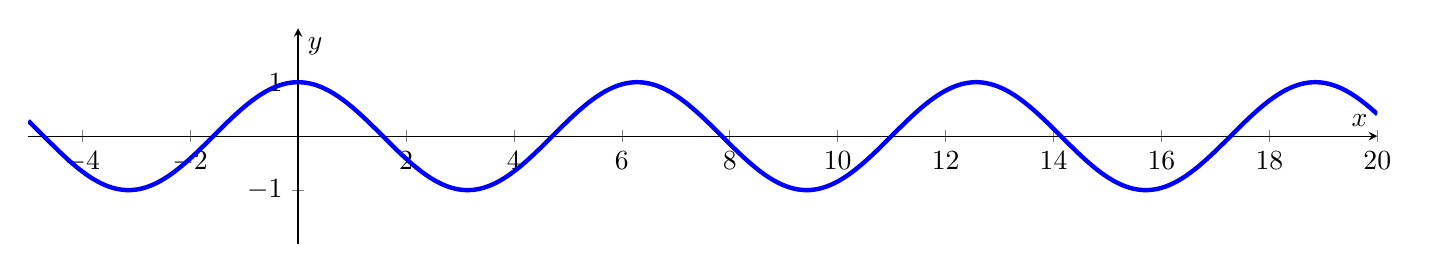
\begin{tikzpicture}
    \begin{axis}[
    scale=2.5,
    axis equal image,
    samples=500,
    axis lines=middle,
    ymin=-2,ymax=2,
    ytick={-1,1},
    ylabel=$y$, 
    xlabel=$x$
    ]
    \addplot[domain=-5:20, black, ultra thick, color=blue] {cos(deg(x))};
    \end{axis}
    \end{tikzpicture}
\end{image}
}

Definitions are displayed using \verb|\begin{definition}| as follows:

\begin{definition}[Absolute value]\label{showcase:absolutevalue}\nl 

	For a real number $a\in\R$, we define the \textit{absolute value} of $a$, denoted $|a|$, as
	\[
		|a| \perdef\displaystyle\ 
		          \left\{
			\begin{array}{rll  } 
				a  & \mbox{if} & a \geq 0 \\
				-a & \mbox{if} & a<0.
			\end{array}\right.
	\]
\end{definition}

Remarks, on the other hand, can simply be included in the running text, or by using \verb|\begin{remark}|:

\begin{remark}[Properties of the absolute value (with $a\in\R$)] \nl
		\begin{enumerate}
			\item Be careful: $|-a|= |a|$, but \textit{definitely not} $\xcancel{|-a|=a}$

			$|-a|=a$ is \textsc{incorrect} if $a<0$. Indeed, if $a=-7$, then $|-a| = |-(-7)| {\color{red}\neq} -7 = a$
			\item $|a^2 + 1| = a^2 + 1$, because $a^2+1$ is always positive.
			% \item $|a^2 - 1| = ....$ \qquad(there is \textsc{no} simple general formula without $|\cdot|$)
\end{enumerate}
\end{remark}

Examples use \verb|\begin{example}|. They can contain online multiple-choice options, which are displayed as regular running text in the PDF.
By default, examples also provide the correct answer in the handout version, while that is not the case for the exercises.

\renewcommand{\choiceminimumverticalsize}{\vphantom{$\sqrt{2}$}} 

\begin{example}[Simple examples of absolute values] \nl 

\begin{xmmulticols}
		\begin{enumerate}
			\item $|5|=5$ and $|-5|=5$
			\item $|\sqrt{2}-1| = $\onlineChoice{\choice[correct]{$\sqrt{2} - 1$}\choice{$1-\sqrt{2}$}}
			\item $|1-\sqrt{2}| = $\wordChoice{\choice[correct]{$\sqrt{2} - 1$}\choice{$1-\sqrt{2}$}}
			\item $|2-\sqrt{2}| = $\wordChoice{\choice{$\sqrt{2} - 2$}\choice[correct]{$2-\sqrt{2}$}}
		\end{enumerate}
\end{xmmulticols}
\end{example}

\begin{exercise}[Simple exercises about absolute values] \nl 

    \begin{xmmulticols}
    \begin{question} $|2-5| = \answer{3}$ \end{question}
    \begin{question} $|5-2| = \answer[onlineshowanswerbutton]{3}$ \end{question}
    \begin{question} $|5-\sqrt{2}| = \answer[onlinenoinput]{3.58578643763}$ \end{question}
    \begin{question} 
        $|1-\sqrt{2}| = $\wordChoice{\choice[correct]{$\sqrt{2} - 1$}\choice{$1-\sqrt{2}$}}
    \end{question}
    \end{xmmulticols}
\end{exercise}


In the PDF, the style can be adjusted using all standard LaTeX possibilities. For the online version, it is possible to add css files:
	\begin{itemize}
		\item \verb|global.css| in the root folder of the repository: all modules in the repository use this styling
		\item \verb|xoursefilename.css| in the folder of the xoursefilename.tex file: all modules in the xourse use this styling
		\item \verb|activityfilename.css| in the folder of the activityfilename.tex file: styling specific to 1 activity.
	\end{itemize}
%	The \verb|ximeraShowcase.css| file specifies in this case that the questions have a purple bar not only on the left but also on the right. 
    % not the case ...?



\end{document}